\chapter{Evaluation}\label{Evaluierung}

Im folgenden Kapitel werden die Ergebnisse der Evaluation von SmartGrazer und dem dazugehörigen kontextabhängigen, sowie dem kontextfreien Payload-Generator vorgestellt. Zunächst wird in Kapitel \ref{eval:BurpSuiteScanner} eine etablierte Anwendung für Websicherheitstest vorgestellt. Anschließend werden die verwendeten Testumgebungen in Kapitel \ref{eval:TestRuns} beschrieben. Danach werden die gesammelten Ergebnisse der Testläufe in Kapitel \ref{eval:ReflectedResultsTestRuns} vorgestellt. Zum Schluss werden in Kapitel \ref{eval:Conclusion} die Ergebnisse der getesteten Anwendungen verglichen, um die Stärken und Schwächen von SmartGrazer und dem Smarty-Generator zu erläutern.

\section{Burp Suite Scanner}\label{eval:BurpSuiteScanner}

Der Burp Suite Scanner wird bei Webseitentests zunächst zwischen die Webseite und den Webbrowser als Proxy geschaltet. Hierdurch können alle Anfragen vom Browser an die Webseite mitgelesen und zurückgehalten werden, was eine genaue Analyse der Anfragen bzw. Antworten ermöglicht.

Bevor die Webanwendung mit der Burp Suite getestet werden kann, muss die Konfiguration des Scanners an die Webseite angepasst werden. Hierzu definiert man zunächst den sogenannten ``Scope''. Dieser bestimmt, welchen Links der Scanner folgen darf, um nach Schwachstellen zu suchen. Wird der Scope zu ungenau definiert, wird der Scanner gegebenenfalls fremde Webseiten testen.

Ist der Scope definiert, kann der Tester im Browser alle zu testenden Links anklicken. Der Scanner prüft die angeklickten Seiten im Hintergrund auf Schwachstellen. Soll eine Webseite genauer untersucht werden, kann diese gesondert an das ``Intruder''-Modul der Testanwendung gesendet werden.

Die Burp Suite erkennt testbare Einstiegspunkte automatisch und markiert diese für den Test. Mit dem Intruder kann der Tester gezielt Payload-Listen für einzelne Parameter durchlaufen, um so weitere Schwachstellen zu finden (siehe Abbildung \ref{fig:BurpSuitebWAPPSniperSettings}).

\begin{figure}[htbp] 
	\centering
	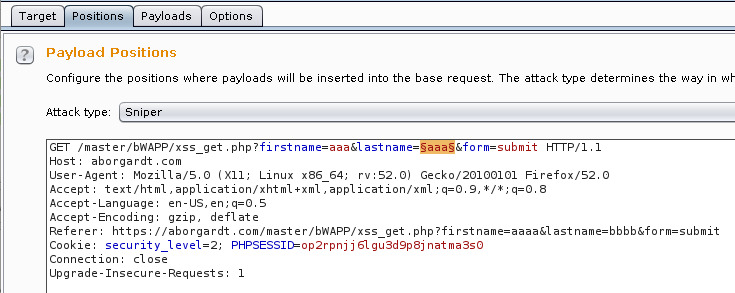
\includegraphics[width=\textwidth]{contents/images/BurpSuitebWAPPSniperSettings}
	\caption{Burp Suite: Konfiguration des Snipers}
	\label{fig:BurpSuitebWAPPSniperSettings}
\end{figure}

Um die Burp Suite als Proxy zu verwenden, muss der Browser mit der entsprechenden Proxy-Adresse konfiguriert werden. Standardmäßig läuft dieser Dienst unter der Adresse 127.0.0.1:8080.

\FloatBarrier
\subsection{Konfiguration}

Für die Evaluation wurde die Burp Suite so konfiguriert, dass diese nur nach reflektierten XSS-Schwachstellen sucht und dementsprechende Payloads verwendet. Die Liste der vorhandenen Typ 1 XSS-Angriffe (Abbildung \ref{fig:BurpSuitebWAPPIntruderSettings}) umfasst nach der Konfiguration insgesamt 20 Payloads.

\begin{figure}[htbp] 
	\centering
	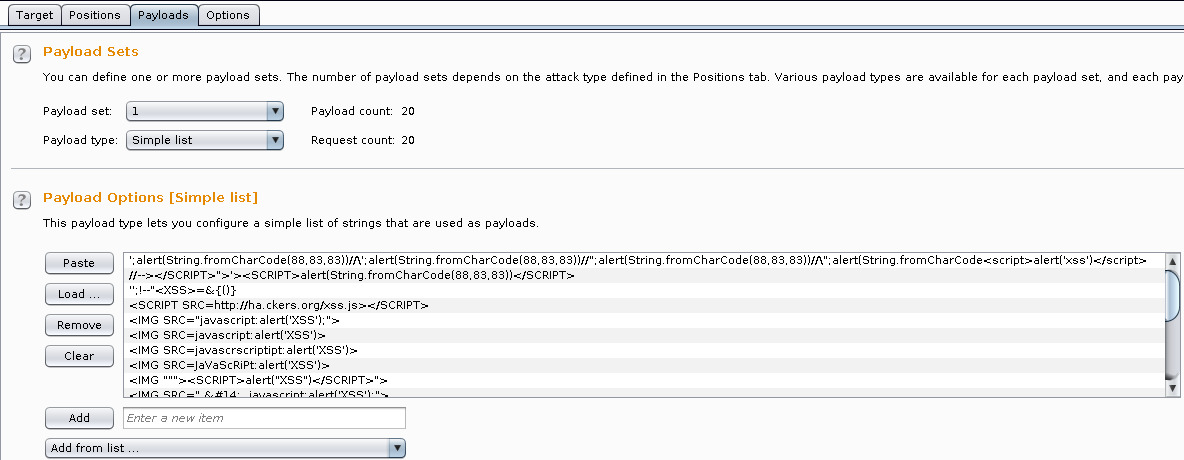
\includegraphics[width=\textwidth]{contents/images/BurpSuitebWAPPIntruderSettings}
	\caption{Burp Suite: Konfiguration des Intruders}
	\label{fig:BurpSuitebWAPPIntruderSettings}
\end{figure}

\newpage

\section{Testdefinition}\label{eval:TestRuns}

\subsection{Erfolgs- und Abbruchkriterium}

Die durchgeführten Testläufe wurden jeweils auf fünf Minuten begrenzt, um eine endlose Ausführung zu vermeiden. 

\subsubsection{Testfall: reflektierte Payloads}

Im Fall der reflektierten Payloads werden solange Payloads gesucht, bis ein vollständig reflektierter Angriff generiert worden ist. Die hier vorgestellten Zahlen beziehen sich auf die Anzahl der getesteten Payloads bis zum ersten reflektierten Payload.

\subsubsection{Testfall: funktionierende Payloads}

Die Generierung von Payloads wird erst abgebrochen, bis der erste reflektierte, ausführbare Payload gefunden worden ist. Hierbei werden neben der Anzahl an Versuchen auch die Anzahl an reflektierten Payloads gezählt, die nicht ausgeführt wurden. Diese Zahl ist ua. ein Indiz für die syntaktische Richtigkeit der generierten Payloads. Durch unterschiedliche Browser-Implementierungen kann syntaktische Validität bei verschiedenen Browsern unterschiedlich interpretiert werden. Die Evaluation verwendete bei den Testläufen den Firefox-Browser bzw. den GeckoDriver aus dem Selenium-Framework\footnote{\url{https://github.com/mozilla/geckodriver/releases/tag/v0.19.0}}.

\FloatBarrier

\subsection{Testapplikationen}

\subsubsection{bWAPP}

\begin{figure}[htp] 
	\centering
	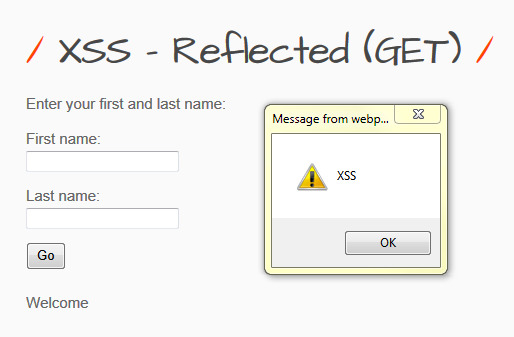
\includegraphics[width=0.5\textwidth]{contents/images/bWAPPExampleImage}
	\caption{bWAPP: XSS-1 Testseite mit Pop-up}
	\label{fig:bWAPPExampleImage}
	\source Quelle: \url{http://itsecgames.blogspot.de/} 
\end{figure}

bWAPP\footnote{\url{http://itsecgames.blogspot.de/}} ist Teil des ``ITSEC Games'' Projekts und beinhaltet über 100 sogenannter Web Bugs. In der Evaluation dieser Arbeit wird ausschließlich gegen die Komponente für reflektiertes XSS getestet.

Wie gut die Webanwendung Benutzereingaben filtert, hängt vom gewählten Sicherheitslevel der Applikation ab. Hier kann zwischen Level 0 bis 2 gewählt werden. Wobei Level 0 keine Änderungen vornimmt. Level 1 die mittels der PHP-Funktion ``addslashes''\footnote{\url{http://php.net/manual/de/function.addslashes.php}} und Level 2 mit der PHP-Funktion ``htmlspecialchars''\footnote{\url{http://php.net/manual/de/function.htmlspecialchars.php}} Benutzereingaben filtert.

Als Zwischenschritt muss sich das zu testende Programm zunächst an der Seite eines Login-Formulars anmelden.

\FloatBarrier
\subsubsection{badWAF}

Um gezielte Testläufe produzieren zu können, wurde die Webanwendung ``badWAF'' im Rahmen dieser Masterthesis implementiert. Ziel der Anwendung ist vor allem die Simulation einer unvollständigen Validierung von Benutzerdaten und Ausgabenkodierung.

Entwickelt wurde eine einfache Webanwendung mit mehreren Seiten. Der Aufbau der einzelnen Seiten ist immer identisch, wie in Abbildung \ref{fig:BadWAFTestFormInputs} dargestellt. Gegeben ist ein Eingabefeld, ein Auswahlfeld für den Kontext und ein Button zum Abschicken der Form. Die bisherige Implementierung umfasst die Kontexte ``HTML'' und ''Attributwert'', sowie das Absenden der Parameter per GET-Methode.

\begin{figure}[htp] 
	\centering
	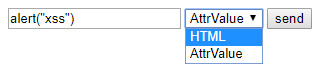
\includegraphics[width=0.5\textwidth]{contents/images/BadWAFTestFormInputs}
	\caption{badWAF: Eingabeformular}
	\label{fig:BadWAFTestFormInputs}
\end{figure}

Das Auswahlfeld für den Kontext bestimmt, in welchem Kontext der gesendete Payload eingebettet wird. Bei der Auswahl des HMTL-Kontexts wird der Payload zwischen zwei div-Tags eingebettet. Im Falle der Attributwert-Auswahl wir der gesendete Wert dem ``value''-Attribut eines input-Tags zugewiesen. Die Abbildungen \ref{fig:BadWAFResultFilterHTML} und \ref{fig:BadWAResultFilterAttrVal} zeigen die Ausgabe des ``fdq''-Filters, welcher alle doppelten Anführungszeichen aus der Benutzereingabe entfernt.

\begin{figure}[htp] 
	\centering
	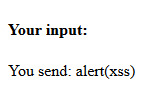
\includegraphics[width=0.3\textwidth]{contents/images/BadWAFResultFilterHTML}
	\caption{badWAF: Antwortseite im HTML-Kontext}
	\label{fig:BadWAFResultFilterHTML}
\end{figure}

\begin{figure}[htp] 
	\centering
	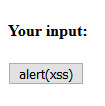
\includegraphics[width=0.2\textwidth]{contents/images/BadWAResultFilterAttrVal}
	\caption{badWAF: Antwortseite im Attributwert-Kontext}
	\label{fig:BadWAResultFilterAttrVal}
\end{figure}

\FloatBarrier
\subsubsection{Einzelfilter}
Jede dieser Seiten beinhaltet einen Filter, der einzelne Elemente aus Payloads entfernt. Die neun implementierten, einfachen Filter werden im Folgenden unter den Abkürzungen aus der unten aufgeführten Liste verwendet.

\begin{description}
	\item[fdq] Entfernen aller doppelten Anführungszeichen.
	\item[fsq] Entfernen aller einfachen Anführungszeichen.
	\item[fpb] Entfernen aller spitzen Klammern.
	\item[fbq] Entfernen aller Backticks.
	\item[fkjs] Entfernen aller Vorkommen des Schlüsselwortes ``javascript''.
	\item[fks] Entfernen aller Vorkommen des Schlüsselwortes ``script'.
	\item[fka] Entfernen aller Vorkommen des Schlüsselwortes ``alert''.
	\item[fts] Entfernen aller Vorkommen der Tags ``<script>'' bzw. ``</script>''.
	\item[fe] Filtern aller JavaScript-Events (Zeichenketten mit dem Muster: ``on....='').
\end{description}

\subsubsection{Kombinierte Filter}
Zu Beginn einer neuen Session wird die Webseite so initialisiert, dass fünf Filterkombinationen zufällig zusammengestellt werden. Bei jeder der fünf Kombinationen wird die Zahl der gewählten Filter um eins erhöht. Dementsprechend wird ein Payload gegen minimal zwei und maximal sechs kombinierte Filter getestet. Hierbei wird eine Kombination sowohl im HTML- als auch im Attributwert-Kontext für einen Payload verwendet.

\section{Ergebnisse}\label{eval:ReflectedResultsTestRuns}

\subsection{Reflektierte Payloads}
\subsubsection{badWAF}

\subsubsubsection{Einfache XSS-Filter}

%Die getesteten Verfahren konnten alle bei den einfachen XSS-Filtern erfolgreich Payloads ermitteln, die komplett reflektiert wurden.
Bei der Verwendung von einfachen XSS-Filtern konnten alle getesteten Verfahren erfolgreich Payloads ermitteln, die vollständig reflektiert wurden.
Alle drei Verfahren haben die meisten Versuche bei dem fpb-Filter benötigt, wie in Abbildung \ref{fig:BadWAFDiagramReflectedFilterHTML} dargestellt. Hierbei konnte die Burp Suite, mit 15 Versuchen, am schnellsten einen passenden Payload finden. Smarty hat, mit 63 Versuchen am längsten benötigt, um einen geeigneten Payload zu erzeugen.

\begin{figure}[htp] 
	\centering
	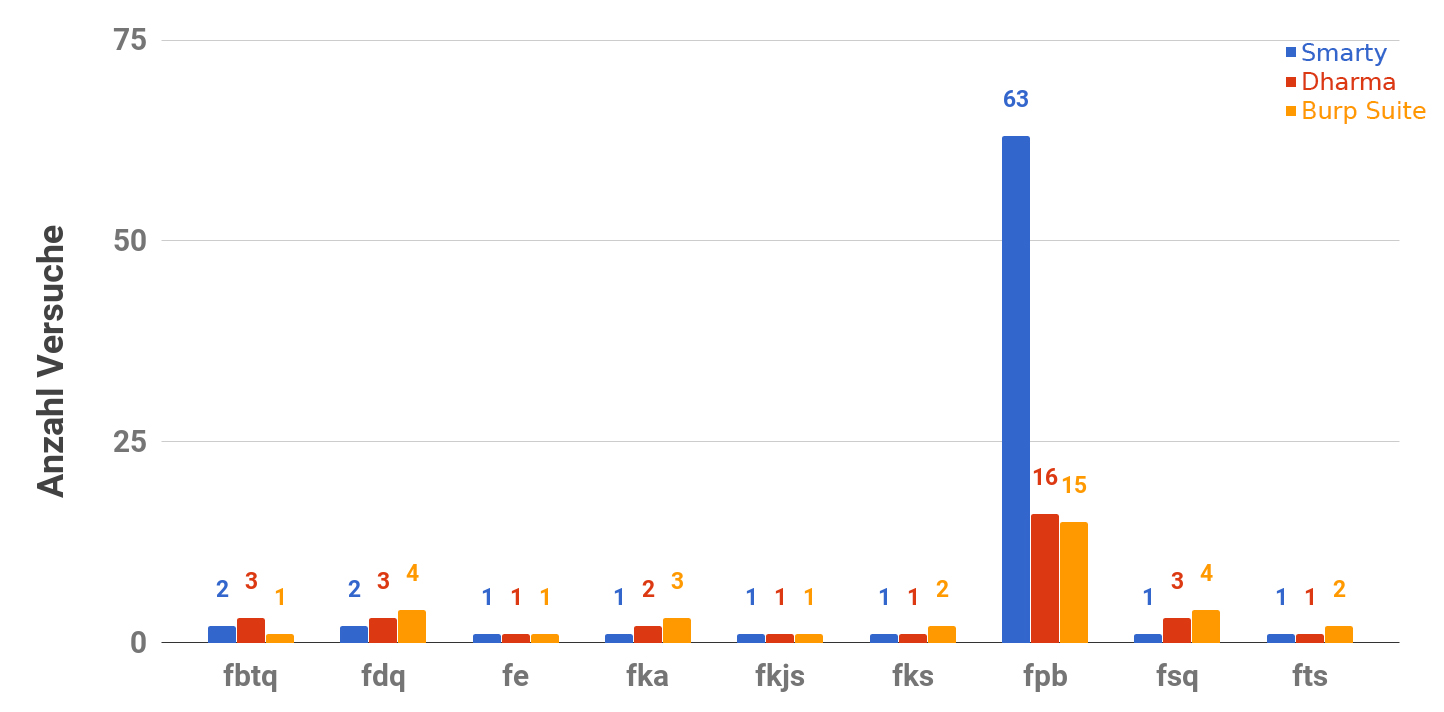
\includegraphics[width=\textwidth]{contents/images/BadWAFDiagramReflectedFilterHTML}
	\caption{badWAF: Durchschnittliche Anzahl der Payloads im HTML-Kontext}
	\label{fig:BadWAFDiagramReflectedFilterHTML}
\end{figure}

In Abbildung \ref{fig:BadWAFDiagramReflectedFilterAttrVal} ist ein ähnliches Ergebnis für die Payloads im Attributwert-Kontext abzulesen. Bei Payload-Generierung für den Attribut-Kontext gelang es Smarty, mit durchschnittlich drei Versuchen weniger einen passenden Payload zu generieren. Dharma und die Burp-Suite konnten im Attribut-Kontext ihre Werte beibehalten.
 
\begin{figure}[htp] 
	\centering
	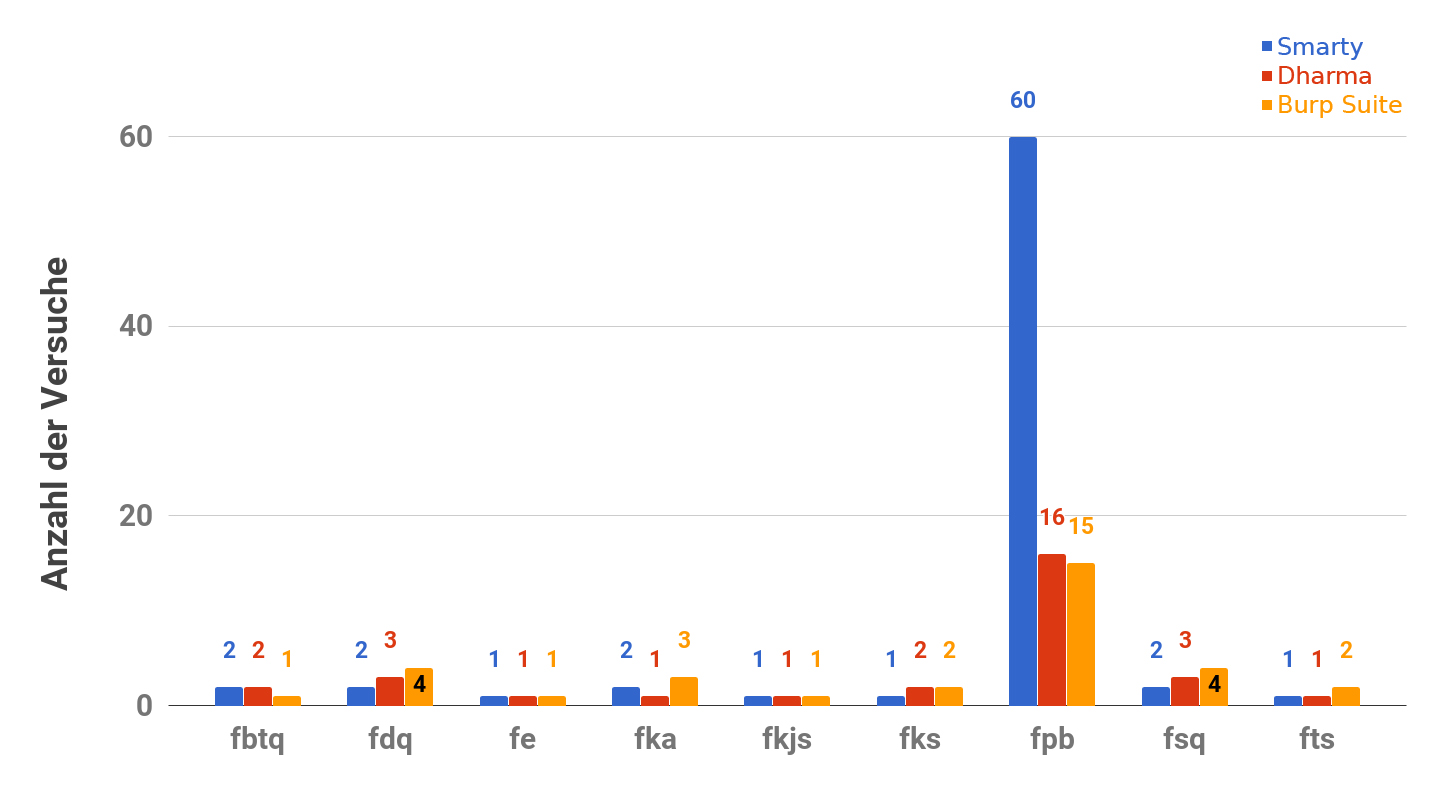
\includegraphics[width=\textwidth]{contents/images/BadWAFDiagramReflectedFilterAttrVal}
	\caption{badWAF: Durchschnittliche Anzahl der Payloads im Attributwert-Kontext}
	\label{fig:BadWAFDiagramReflectedFilterAttrVal}
\end{figure}
\FloatBarrier

Abbildung\footnote{Die Payloads wurden wegen möglichen Steuerzeichen aus einem Texteditor abfotografiert.} \ref{fig:BadWAFreflectedResultsSingleFPB} zeigt eine zufällige Auswahl an erfolgreich reflektierten Payloads mit aktivem fpb-Filter im HTML-Kontext. Erkennbar ist vor allem die Tendenz ein bestimmtes Angriffsmuster, mit verschiedenen Outbreak-Sequenzen, zu verwenden. Durch den aktiven Filter wurden verstärkt Payloads generiert, die in einem JavaScript-Kontext funktioniert hätten, jedoch im HTML-Kontext wirkungslos bleiben.

\begin{figure}[htp] 
	\centering
	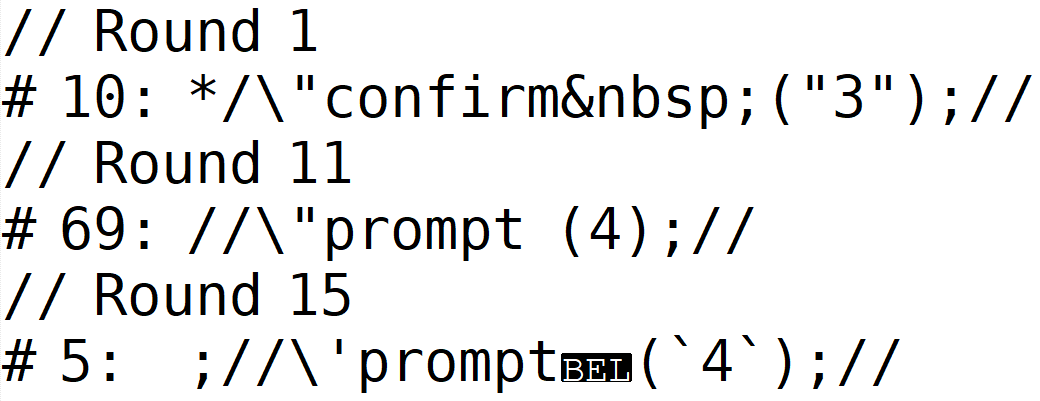
\includegraphics[width=.60\textwidth]{contents/images/BadWAFreflectedResultsSingleFPB}
	\caption{Smarty: Reflektierte Payloads mit aktivem fpb-Filter}
	\label{fig:BadWAFreflectedResultsSingleFPB}
\end{figure}

Alternativ wird in Abbildung \ref{fig:BadWAFReflectedResultsSingleFKJS} eine Auswahl erzeugter Payloads mit aktivem fkjs-Filter im HTML-Kontext dargestellt. Durch eine größere Musterbasis variieren die erzeugten Payloads stärker.

\begin{figure}[htp] 
	\centering
	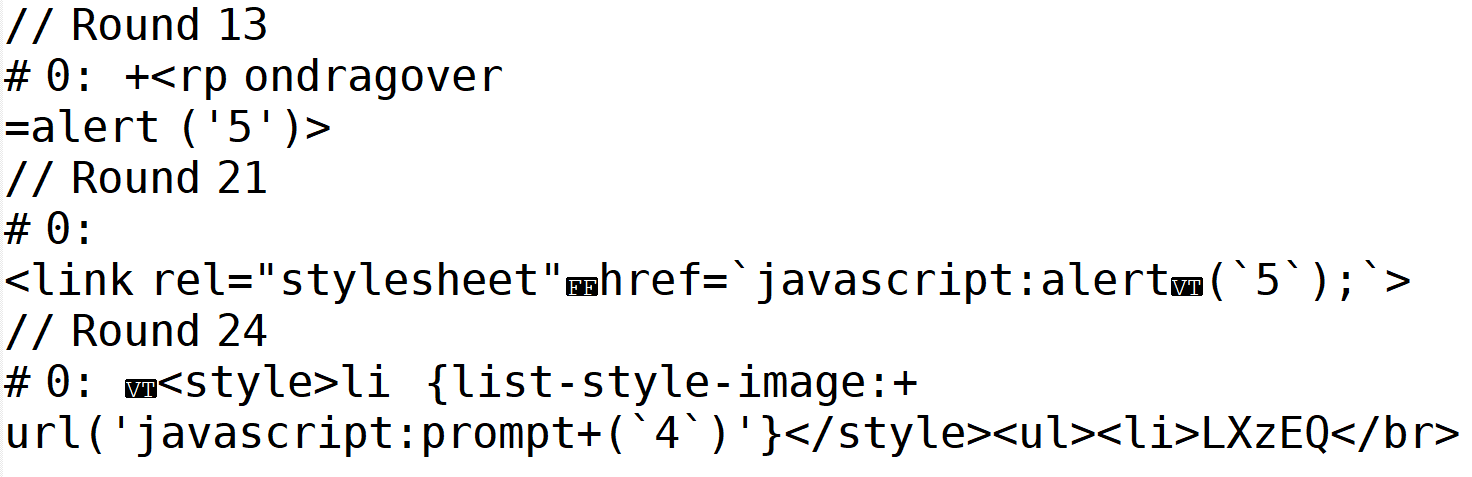
\includegraphics[width=\textwidth]{contents/images/BadWAFReflectedResultsSingleFKJS}
	\caption{Smarty: Reflektierte Payloads mit aktivem fkjs-Filter}
	\label{fig:BadWAFReflectedResultsSingleFKJS}
\end{figure}
\FloatBarrier

\subsubsubsection{Kombinierte XSS-Filter}

Bei den Testläufen mit kombinierten XSS-Filtern hat Smarty in allen Durchläufen einen reflektierenden Payload gefunden. Sowohl Dharma als auch die Burp Suite konnte bei einigen Kombinationen keinen Payload ermitteln.

%Dharma ist bei zwei Testläufen (fünf und sechs kombinierte Filter) innerhalb des Zeitlimits keinen passenden Payload finden können. 
Für Dharma war es bei Testläufen (fünf und sechs kombinierte Filter) nicht möglich, innerhalb des Zeitlimits von fünf Minuten einen passenden Payload zu finden. Die Burp Suite konnte mit steigenden Filterkombinationen immer weniger Payloads reflektieren.

%Der Verlauf der Zuverlässigkeiten ist in den Abbildungen  \ref{fig:BadWAFDiagramReflectedFilterHTMLCombined} und \ref{fig:BadWAFDiagramReflectedFilterAttrValCombined} zeigt den Verlauf der Zuverlässigkeit für die verwendeten Programme, einen reflektierten Payload zu finden\footnote{Der blaue Strich von Smarty wird in diesem Diagramm vollständig vom roten Überdeckt.}.

Der Verlauf der Zuverlässigkeit ist in den Abbildung \ref{fig:BadWAFDiagramReflectedFilterHTMLCombined} und \ref{fig:BadWAFDiagramReflectedFilterAttrValCombined} dargestellt. Dabei beziehen sich die Diagramme auf die verschiedenen getesteten Kontexte.
Sowohl Smarty als auch Dharma haben im HTML-Kontext in jedem Testlauf einen reflektierten Payload erzeugen können. Die Burp Suite konnte mit der gegebenen Liste schon bei zwei kombinierten Filtern, bei drei Durchgängen keinen passenden Angriff finden.

\begin{figure}[htbp] 
	\centering
	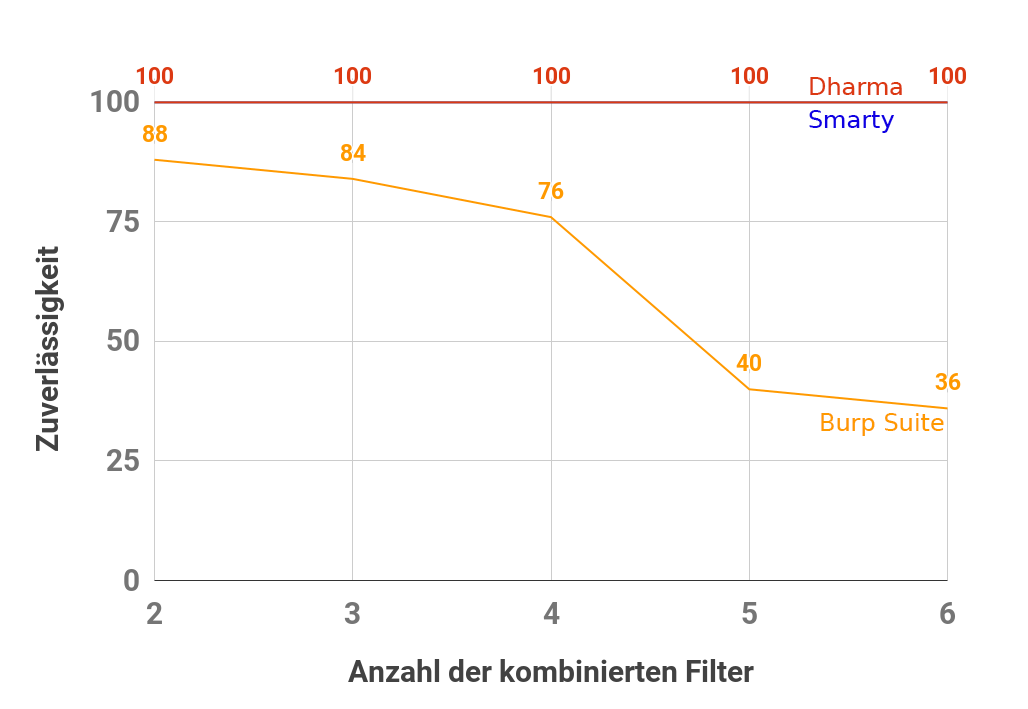
\includegraphics[width=0.8\textwidth]{contents/images/BadWAFDiagramReflectedFilterHTMLCombined}
	\caption{badWAF: Zuverlässigkeit für reflektierte Payloads im HTML-Kontext}
	\label{fig:BadWAFDiagramReflectedFilterHTMLCombined}
\end{figure}

Im Attributwert-Kontext konnte Dharma bei zwei der 25 Durchläufe keinen passenden Payload innerhalb der gegebenen Zeitvorgabe konstruieren. Der Smarty-Generator hingegen konnte eine 100\%-ige Zuverlässigkeit vorweisen.

\begin{figure}[htbp] 
	\centering
	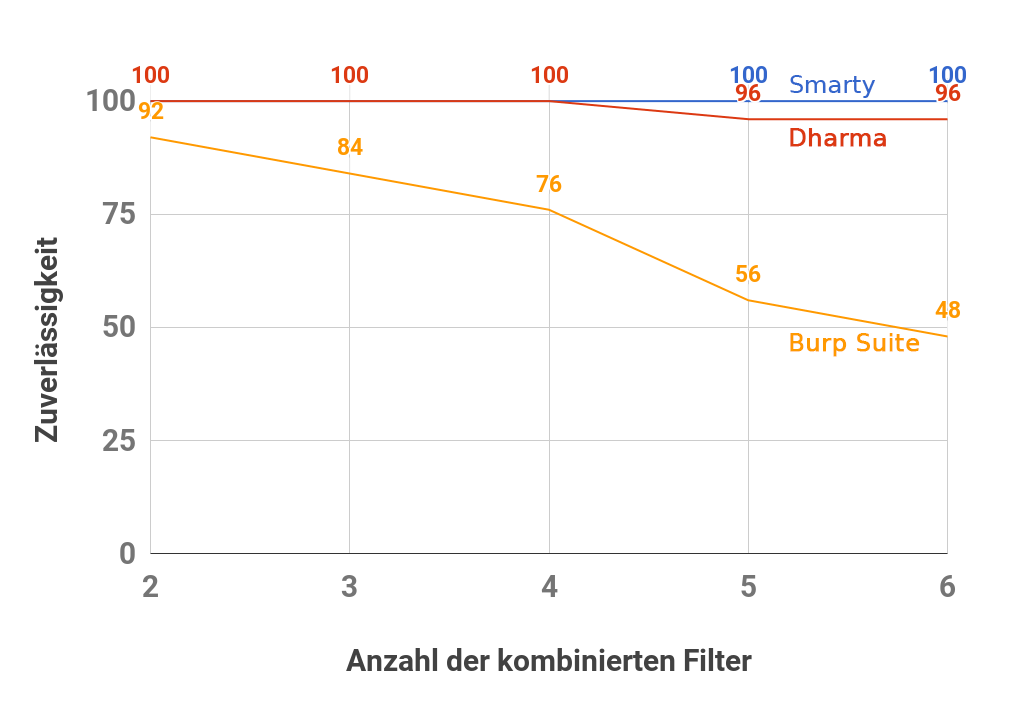
\includegraphics[width=.8\textwidth]{contents/images/BadWAFDiagramReflectedFilterAttrValCombined}
	\caption{badWAF: Zuverlässigkeit für reflektierte Payloads im Attributwert-Kontext}
	\label{fig:BadWAFDiagramReflectedFilterAttrValCombined}
\end{figure}

\FloatBarrier
In Abbildung \ref{fig:BadWAFReflectedResultsCombined} ist eine Auswahl reflektierter Payloads aus verschiedenen Testläufen mit verschiedenen Filterkombinationen dargestellt. Wie bereits erwähnt wird die Generation von Smarty durch bestimmte Filterkombinationen dazu gebracht einen Payload mit wenig Elementen zu wählen, die jedoch noch (relativ) viele Lebenspunkte besitzen. So wird eine Reflexion erreicht, die keine Ausführung des Codes ermöglicht.

\begin{figure}[htbp] 
	\centering
	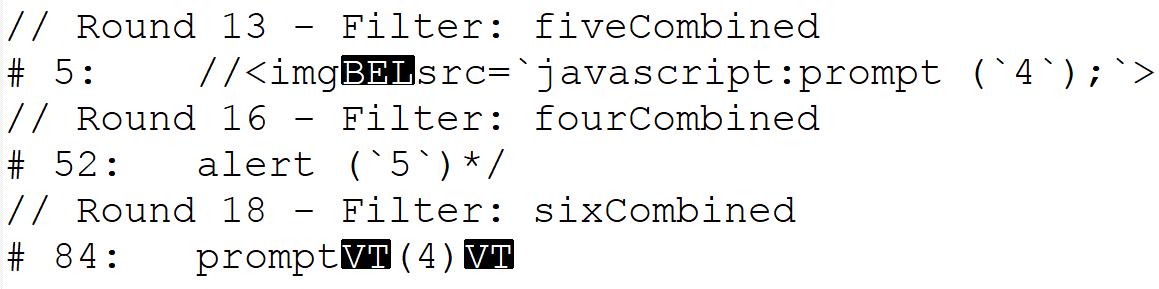
\includegraphics[width=\textwidth]{contents/images/BadWAFReflectedResultsCombined}
	\caption{Smarty: Reflektierte Payloads mit kombinierten Filtern}
	\label{fig:BadWAFReflectedResultsCombined}
\end{figure}


\FloatBarrier

\subsubsection{bWAPP}

Die Testläufe gegen die bWAPP-Anwendung wurden mit den drei beschriebenen Sicherheitsleveln durchgeführt. Bei Durchgängen mit der niedrigsten Sicherheitsstufe (Level 0) konnten alle drei Verfahren den ersten gesendeten Payload reflektieren.

Auf Level eins konnte die Burp Suite mit durchschnittlich vier Payloads einen Payload reflektieren. Smarty belegte mit sechs Payloads den zweiten Platz. Schlusslicht wurde der Dharma-Generator mit zehn Payloads. In Abbildung \ref{fig:bWAPPLvl1ReflectedTries} ist deutlich zu sehen, welchen Vorteil das Verwenden von statischen Listen hat. Bis auf wenige Ausnahmen konnte die Burp Suite immer die geringste Anzahl an benötigten Payloads aufweisen. Bemerkenswert ist auch die extreme Schwankung der Versuche bei der kontextfreien Generierung von Dharma.
 

\begin{figure}[htbp] 
	\centering
	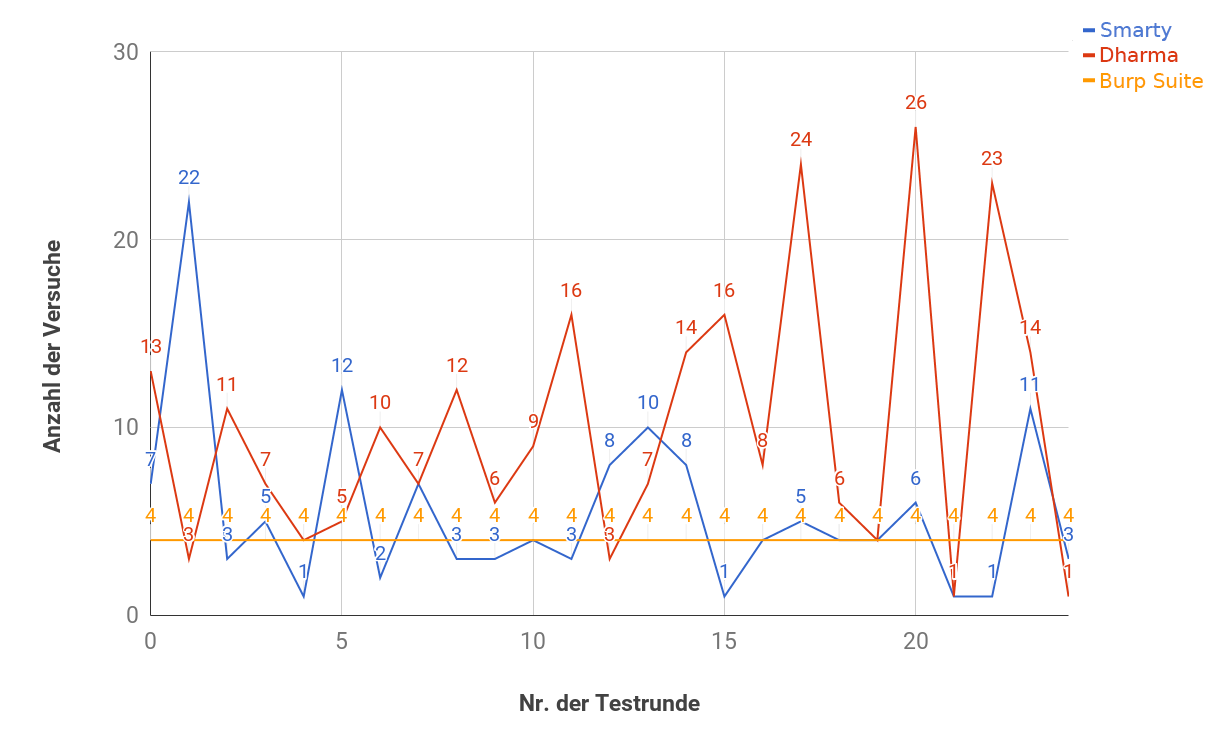
\includegraphics[width=\textwidth]{contents/images/bWAPPLvl1ReflectedTries}
	\caption{bWAPP: Verlauf der Versuche für Level 1}
	\label{fig:bWAPPLvl1ReflectedTries}
\end{figure}

%Die Sicherheitsstufe zwei konnte alle Angriffe der Burp Suite-Liste erfolgreich filtern.  32\% der generierten Payloads von Dharma wurden erfolgreich von der bWAPP-Webanwendung reflektiert.
Im abschließenden Testlauf mit Sicherheitsstufe zwei konnte bWAPP alle Payloads der Burp Suite erfolgreich filtern. Im Vergleich dazu erreichte Dharma eine Quote an erfolgreich reflektierten Payloads von 32\%. Die meisten reflektierten Payloads konnte Smary generieren. Hier konnten 80\% der generierten Payloads in der Antwort der Webseite gefunden werden. Der Verlauf der benötigten Versuche in Abbildung \ref{fig:bWAPPLvl2ReflectedTries} zeigt wieder, dass die Zahl der getesteten Payloads enorm ansteigen kann. Sowohl Smarty, als auch Dharma haben im zweiten Testlauf eine erhöhte Zahl getesteter Payloads benötigt. Durch diese hohe Testabdeckung können aber dennoch Payloads gefunden werden, die trotz einer starken Prüfung reflektiert werden.


\begin{figure}[htbp] 
	\centering
	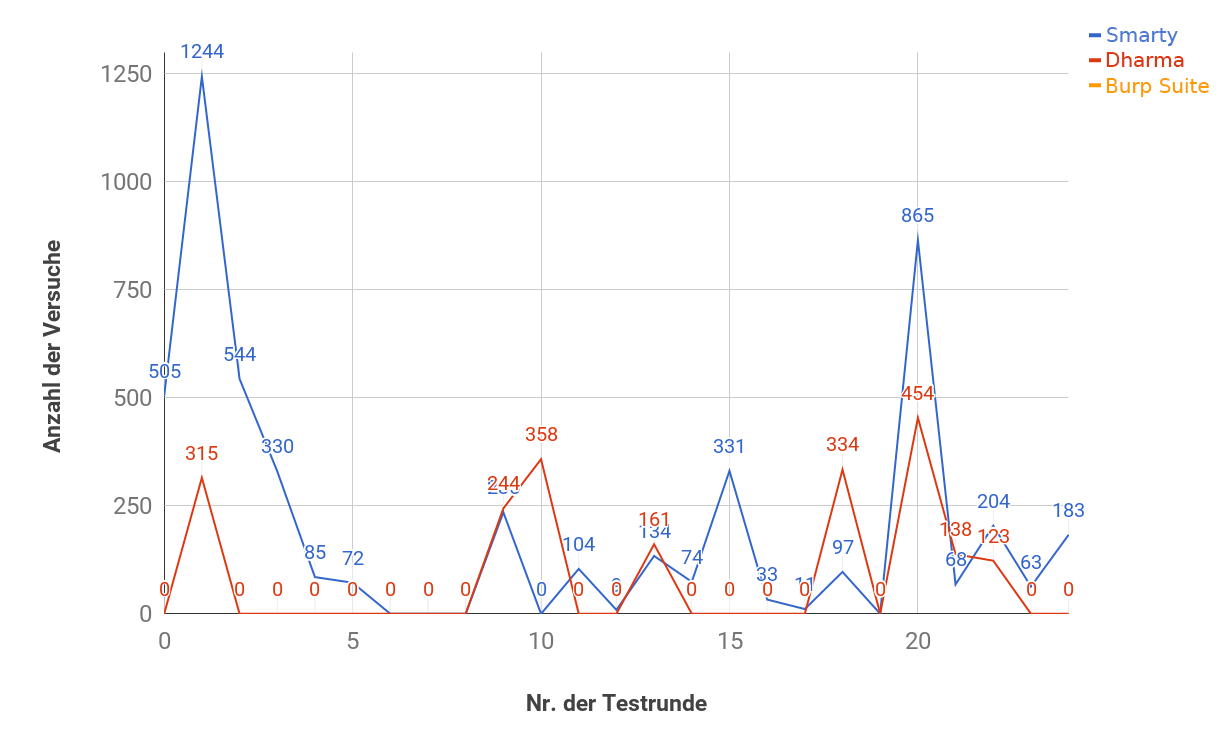
\includegraphics[width=\textwidth]{contents/images/bWAPPLvl2ReflectedTries}
	\caption{bWAPP: Verlauf der Versuche für Level 2}
	\label{fig:bWAPPLvl2ReflectedTries}
\end{figure}

\FloatBarrier
\subsection{Ausgeführte Payloads}

\subsubsection{Generierung ausführbarer Payloads}

In einem weiteren Schritt wurde evaluiert, wie effektiv die generierten Payloads von Smarty, Dharma und der Burp Suite sind. Hierzu wurden zehn Generierungsrunden durchgeführt und geprüft ob der verwendete Payload beim Laden der Webseite im Browser ausgeführt wurde.

\subsubsubsection{badWAF}

Als besondere Schwäche der Generatoren kann wieder der \textbf{fpb}-Filter identifiziert werden. Keiner der verwendeten Genetaroren/Listen konnte einen erfolgreich ausgeführten Payload für diesen Filter finden. SmartGrazer generierte durchschnittlich über 6000 Payloads für diesen Filter, von denen 43 Payloads im HTML-Kontext und 48 Payloads im Attributwert-Kontext erfolgreich reflektiert worden sind.

Die Abbildungen \ref{fig:badWAF-html-execute-combined} und \ref{fig:badWAF-attrval-execute-combined} zeigen, wie die Zuverlässigkeiten mit steigender, kombinierter Filterzahl verlaufen. Während Smarty und die Burp Suite es schafften, einige Payloads zur Ausführung zu bringen, kann bei Dharma eine deutliche Schwäche diesbezüglich beobachtet werden. Besondere Schwierigkeiten hat Dharma hier bei fünf und sechs kombinierten Filtern.

\begin{figure}[htbp] 
	\centering
	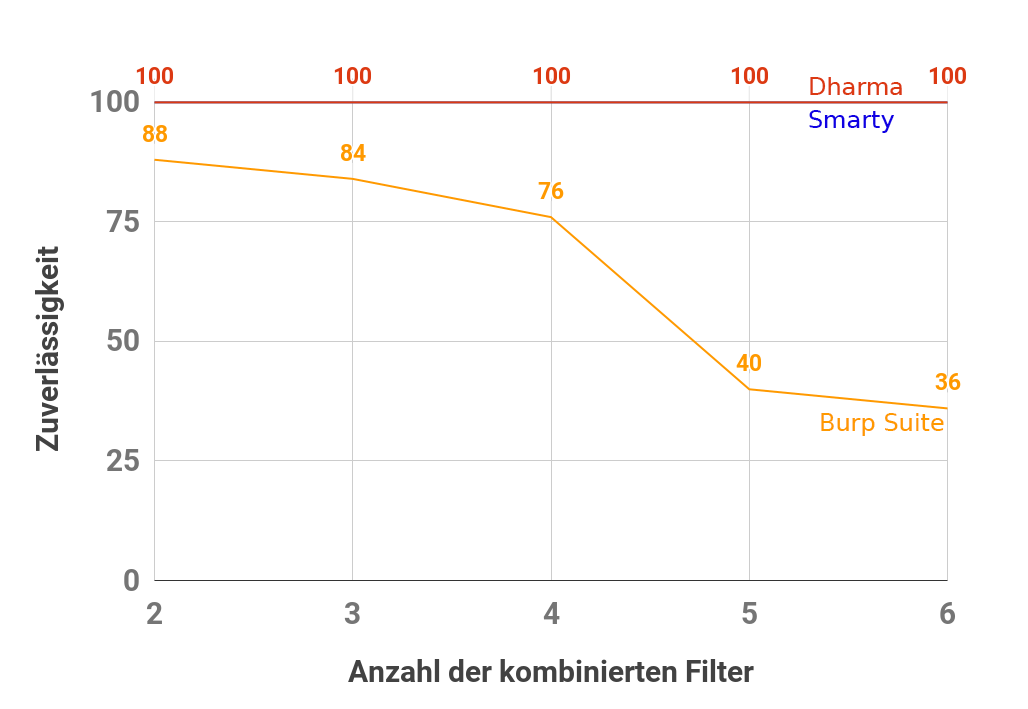
\includegraphics[width=\textwidth]{contents/images/BadWAFDiagramReflectedFilterHTMLCombined}
	\caption{badWAF: Zuverlässigkeit für ausführbare Payloads im HTML-Kontext}
	\label{fig:badWAF-html-execute-combined}
\end{figure}

\FloatBarrier
Während Smarty bei allen Filterkombinationen einen funktionierenden Payload für den HTML-Kontext generieren konnte, fällt die Zuverlässigkeit der anderen Verfahren besonders im Attributwert-Kontext merklich ab. Ein Grund hierfür kann die bestehende Auswahl an Grammatikdefinitionen sein.

\begin{figure}[htbp] 
	\centering
	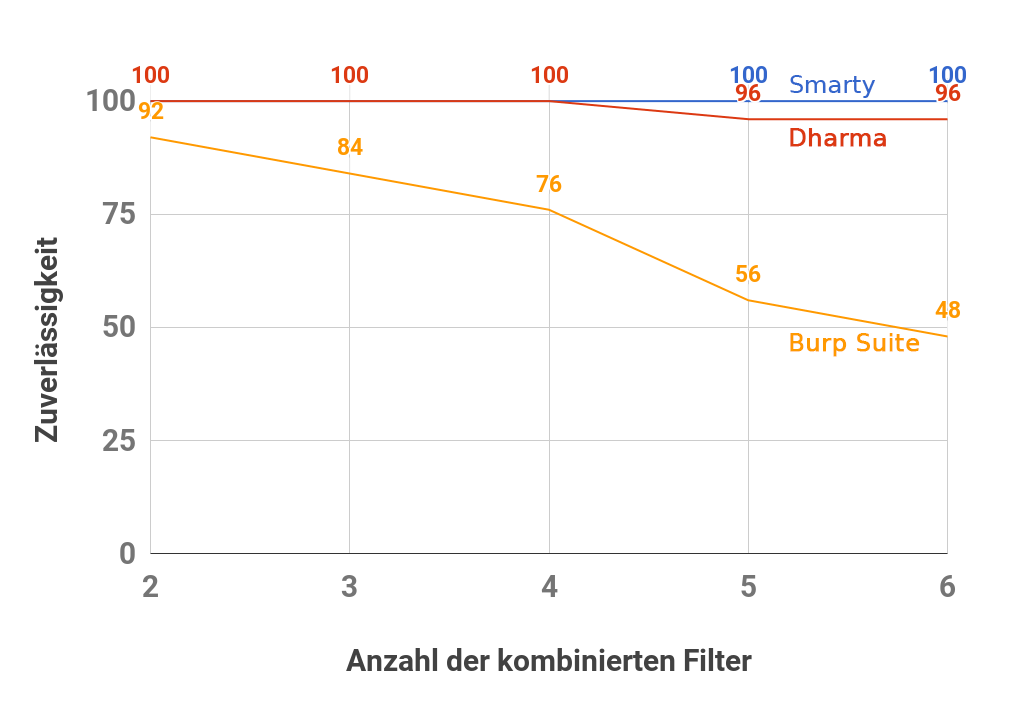
\includegraphics[width=\textwidth]{contents/images/BadWAFDiagramReflectedFilterAttrValCombined}
	\caption{badWAF: Zuverlässigkeit für ausführbare Payloads im AttrVal-Kontext}
	\label{fig:badWAF-attrval-execute-combined}
\end{figure}

\subsubsubsection{bWAPP}\label{ssec:evaluation-executed-bwapp}

Smarty und die Burp Suite konnten auf Level 0 und 1 eine Zuverlässigkeit von 100\% erreichen. Einen besonderer Fall konnte bei einem Payload der Burp Suite beobachtet werden. Hier wurde ein Payload ausgeführt, der vorher von der SUT manipuliert worden ist. Der betroffene Payload enthielt die Zeichenkette ``javajavascriptscript'', welche nach dem entfernen von ``javascript'' wiederum ein valides Stück JavaScript-Code ergab. Diese Fähigkeit der Mutation ist in Smarty bisher nicht implementiert worden. 

Dharma hatte wiederholt bei der Generierung von funktionierendem Quellcode Probleme, was auf die kontextfreie Eigenschaft des Generators zurückzuführen ist. Besonders in der niedrigsten Sicherheitsstufe konnte Dharma nur eine Zuverlässigkeit von 48\% erreichen. Dieser Wert stieg bei Sicherheitsstufe 1 wieder auf 76\%.

In den Abbildungen \ref{fig:bWAPPLvl0ExecutedTries} und \ref{fig:bWAPPLvl1ExecutedTries} sind die benötigten Versuche für die Sicherheitslevel null und eins dargestellt. Deutlich wird auf beiden Abbildungen, dass Smarty in diesen Tests mit Abstand weniger Versuche benötigte als Dharma.

Auf Level 0 konnte die Burp Suite und der verwendete JavaScript-Polyglott jeweils eine sofortige Ausführung erreichen. Daher wurde die Burp Suite in Abbildung \ref{fig:bWAPPLvl1ExecutedTries} weggelassen.

\begin{figure}[htbp] 
	\centering
	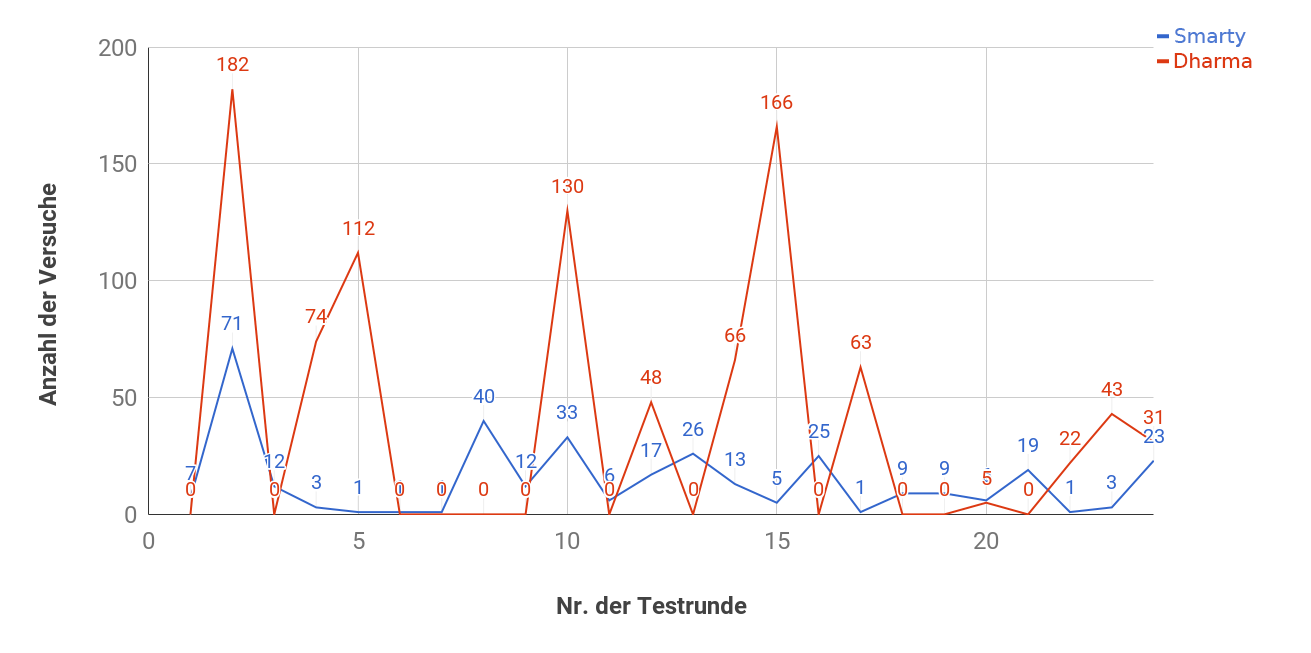
\includegraphics[width=\textwidth]{contents/images/bWAPPLvl0ExecutedTries}
	\caption{bWAPP: Verlauf der Versuche für ausgeführte Payloads auf Level 0}
	\label{fig:bWAPPLvl0ExecutedTries}
\end{figure}

\begin{figure}[htbp] 
	\centering
	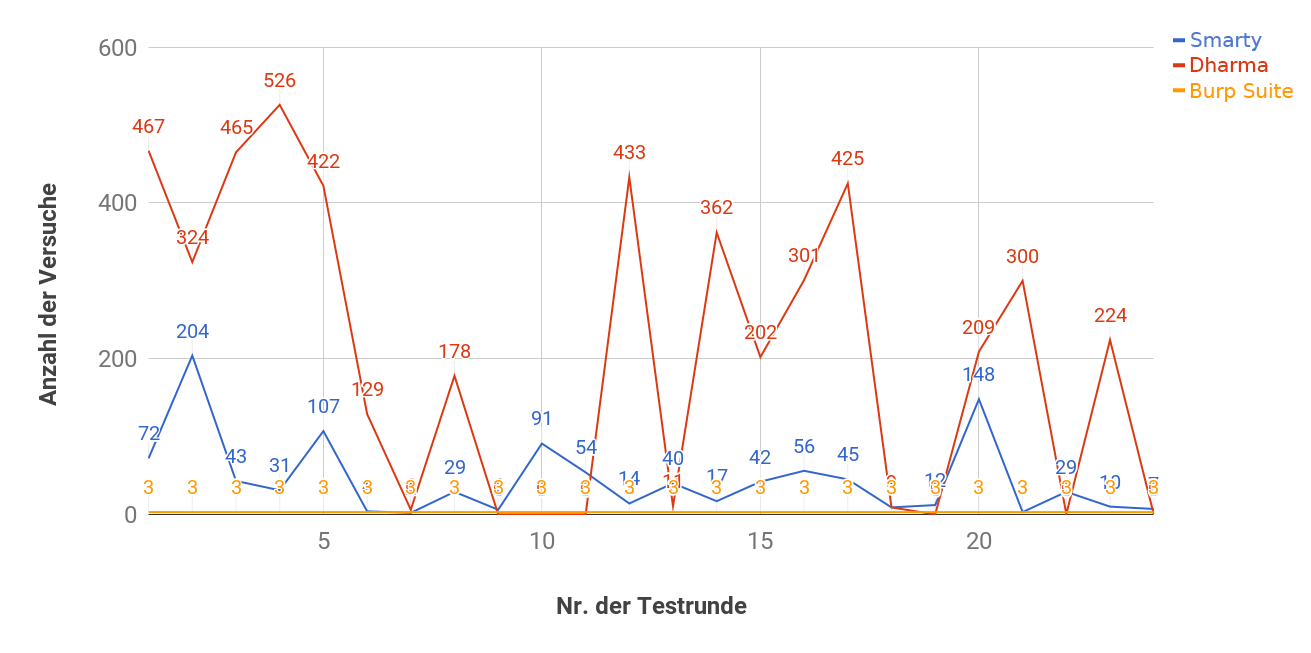
\includegraphics[width=\textwidth]{contents/images/bWAPPLvl1ExecutedTries}
	\caption{bWAPP: Verlauf der Versuche für ausgeführte Payloads auf Level 1}
	\label{fig:bWAPPLvl1ExecutedTries}
\end{figure}

Zum Vergleich der erzeugten Payloads sind in Abbildung \ref{fig:bWAPPExecutedResultsLevel1} exemplarisch zwei von Smarty und Dharma generierte Payloads dargestellt. Beide Payloads führten während des Tests zu einer Ausführung des enthaltenen JavaScript-Codes.

\begin{figure}[htbp] 
	\centering
	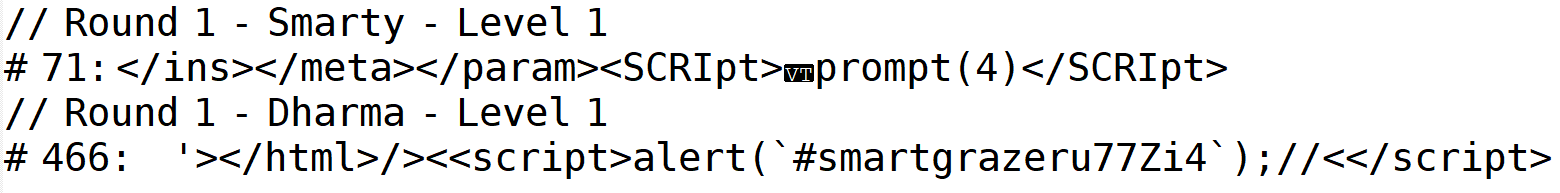
\includegraphics[width=.9\textwidth]{contents/images/bWAPPExecutedResultsLevel1}
	\caption{bWAPP: Ausgeführte Payloads auf Level 1}
	\label{fig:bWAPPExecutedResultsLevel1}
\end{figure}


\FloatBarrier
\section{Fazit}\label{eval:Conclusion}


%Die besonders deutliche Schwäche von SmartGrazer im Bezug auf die gefilterten spitzen Klammern, offenbart Optimierungspotential der aktuellen Implementierung. Denkbar wäre eine neue Mutator-Klasse, welche die gefilterten Zeichen in andere Formate kodiert.

Wie die Testläufe auf den vorherigen Seiten gezeigt haben, offenbart SmartGrazer vor allem in Bezug auf die gefilterten spitzen Klammern Optimierungspotentiale. Mögliches Verbesserungspotential könnte ggf. die Einführung einer neuen Mutator-Klasse sein, die die gefilterten Zeichen in andere Formate kodiert.

Tendenziell benötigte Dharma im Durchschnitt weniger Payloads, um passende Payloads zu konstruieren. Ein möglicher Grund hierfür könnte eine für SmartGrazer unvorteilhafte Filterkombination sein. Wie bereits erkannt, hat Smarty Probleme mit dem Filter für spitze Klammern. Falls dieser Filter in der zufälligen Auswahl für Smarty gewählt wurde, kann dies dessen Ergebnis zum Negativen verändern. Diesen Umstand kann man bei zukünftigen Testläufen genauer analysieren, um die Effizienz weiter zu steigern.

Zusammengefasst konnte Smarty mit einer Zuverlässigkeit von 93\% einen reflektierten Payload gegen bWAPP konstruieren. Auch Dharma erreichte eine höhere Zuverlässigkeit von 77\%, gegenüber der Burp Suite mit 67\%. Letztendlich kann gesagt werden, dass Smarty in den meisten Fällen einen erfolgreich reflektierten Payload konstruieren kann, wenn eine kombinatorische Möglichkeit vorhanden ist. Wie viele falsch-positive Resultate hierbei generiert werden, wurde in dieser Arbeit nicht geprüft.

Jedoch wurde durch Testläufe, bei denen ein funktionierender Payload gesucht wurde, die Existenz erfolgreich generierter Payloads bestätigt. Dabei handelt es sich jedoch nur um eine Untergruppe der tatsächlich funktionierenden Payloads, da viele JavaScript-Events ein manuelles Ausführen erfordern.

Smarty konnte mit einer Zuverlässigkeit von insgesamt 66\% einen ausführbaren Payload generieren und testen. Hierbei wurde bei Tests im HTML-Kontext eine Zuverlässigkeit von 82\% erreicht. Im Attributwert-Kontext konnte hingegen nur eine Zuverlässigkeit von 50\% erreicht werden. Gerade im Bereich anderer Kontexte besteht daher noch viel Raum für Verbesserungen.
